% \Image{Capa do livro (; )}{PNLD2022-017-01.png}
% \Image{Foto do Autor (Arquivo do autor)}{PNLD2022-017-02.png}
% \Image{Foto do Ilustrador (Arquivo do autor)}{PNLD2022-017-03.png}
% \Image{Ilustração do livro (; )}{PNLD2022-017-04.png}
% \Image{Ilustração do livro (; )}{PNLD2022-017-05.png}
% \Image{Ilustração do livro (; )}{PNLD2022-017-06.png}



\documentclass[11pt]{extarticle}
\usepackage{manualdoprofessor}
\usepackage{fichatecnica}
\usepackage{lipsum,media9}
\usepackage[justification=raggedright]{caption}
\usepackage[one]{bncc}
\usepackage[lunna]{../edlab}
\usepackage{marginnote}
\usepackage{pdfpages}
\usepackage[printwatermark]{xwatermark}
\newwatermark[pagex=2]{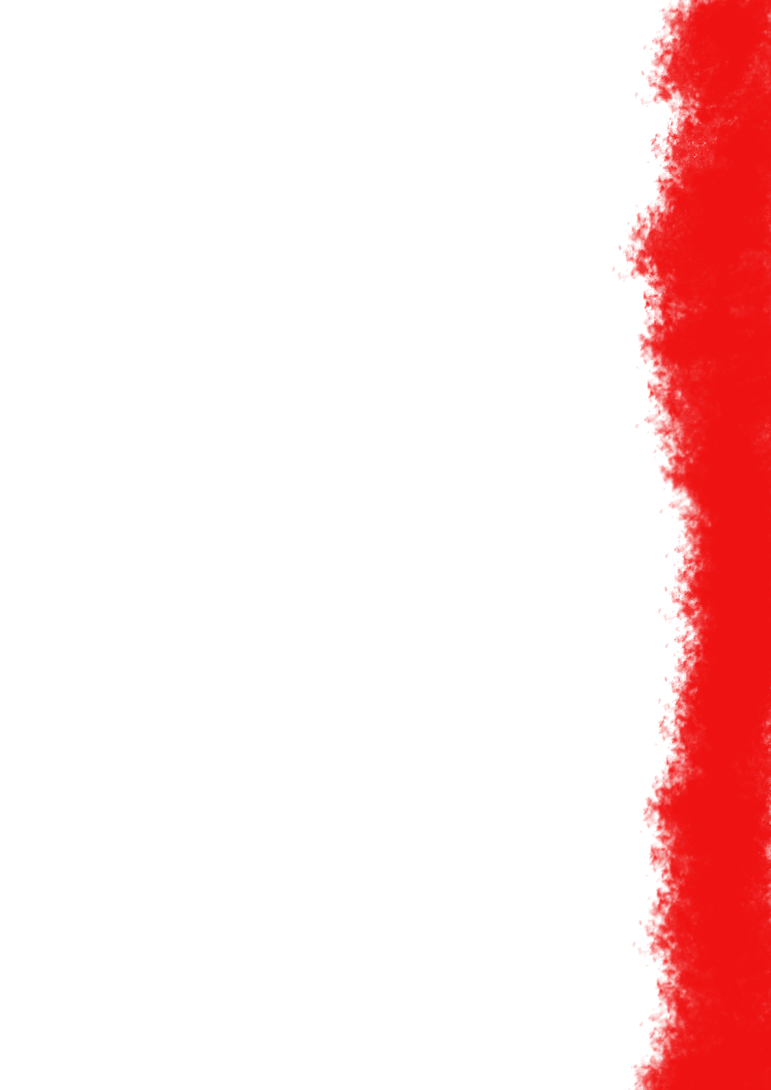
\includegraphics[scale=3.3]{watermarks/test-a.png}}	% página específica
%\newwatermark[oddpages]{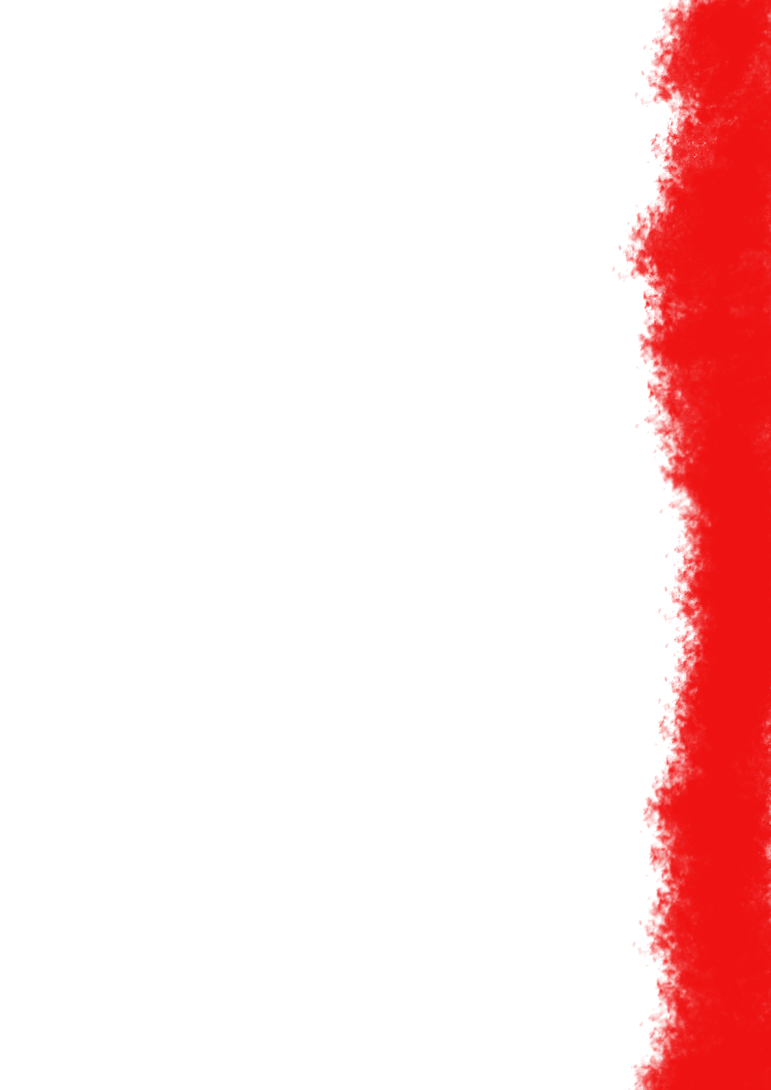
\includegraphics{watermarks/test-a.png}}			% páginas ímpars
%\newwatermark[evenpages]{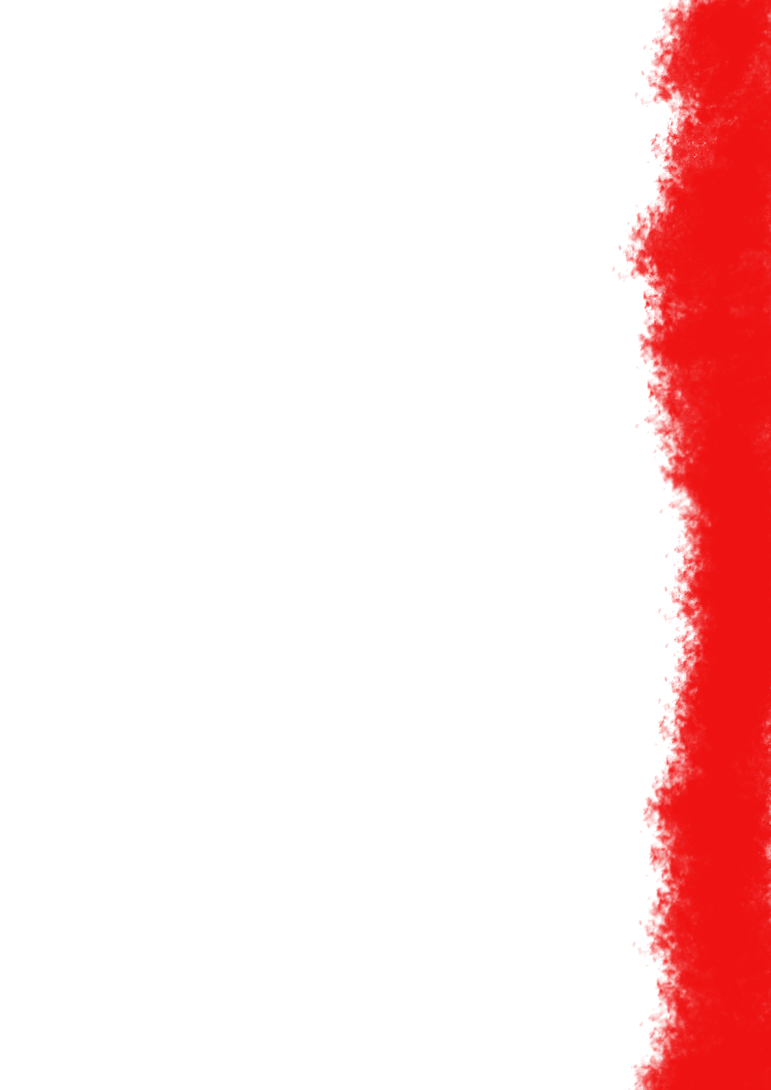
\includegraphics{watermarks/test-a.png}}			% págimas pares
\newwatermark[allpages]{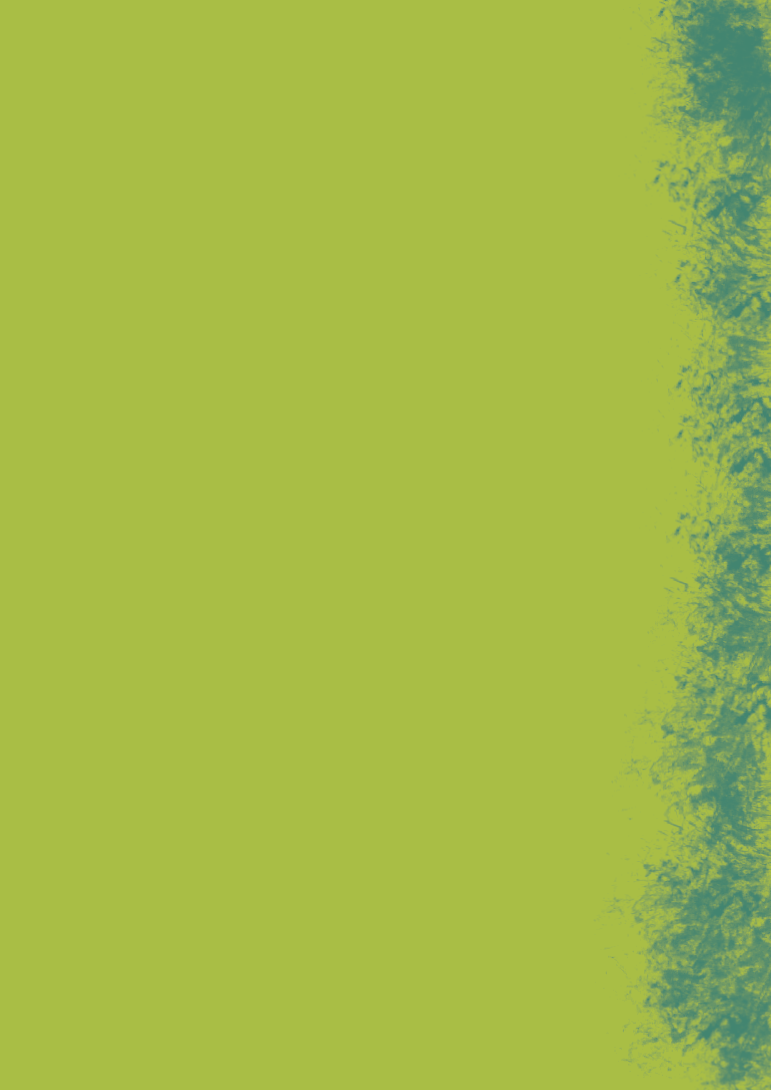
\includegraphics[scale=3.3]{watermarks/test-b.png}}

\pagecolor{cyan!0!magenta!10!yellow!28!black!28!}

\newcommand{\AutorLivro}{Lucas-K}
\newcommand{\TituloLivro}{O caminho das letras}
\newcommand{\Tema}{Jogos; brincadeiras e diversão}
\newcommand{\Genero}{Narrativos: fábulas originais; da literatura universal e da tradição popular; etc}
\newcommand{\imagemCapa}{./images/PNLD2022-017-01.pdf}
\newcommand{\issnppub}{978-65-89705-05-5}
\newcommand{\issnepub}{978-65-89705-07-9}
% \newcommand{\fichacatalografica}{PNLD0001-00.png}
\newcommand{\colaborador}{{Paulo Pompermaier e Renier Silva}}

\begin{document}

\title{\TituloLivro}
\author{\AutorLivro}
\def\authornotes{\colaborador}

\date{}
\maketitle

%\begin{abstract}\addcontentsline{toc}{section}{Carta ao professor}
%\pagebreak

\tableofcontents



\section{Sobre o livro}

%27 caracteres
\paragraph{O livro} 
``O caminho das letras'' é um livro composto por textos,
ilustrações e jogos interativos. 
%822 caracteres
\paragraph{Descrição} 
Cada página do livro apresenta uma nova letra do alfabeto de forma lúdica.
A narrativa é sobre letras que foram passear em diferentes lugares e a 
criança deve encontrá-las riscando o papel.
%411 caracteres
\paragraph{Competências} 
O livro ``O caminho das letras'' trabalha competências de espacialidade como
as noções de em cima, embaixo, no meio, atrás etc. que fazem parte
deste momento de desenvolvimento das crianças na \textbf{Pré-escola}.
Também a coordenação motora é trabalhada no manejo do lápis para
riscar o trajeto entre a pessoa e a letra. Além disso, as crianças
são apresentadas ao alfabeto da língua portuguesa, etapa fundamental
no contato com a escrita. 
%862 caracteres
\paragraph{Aprofundamento} 
Este material tem a intenção de contribuir para que você consiga desenvolver um trabalho aprofundado 
com esta obra na sala de aula. Você encontrará informações sobre o autor, sobre 
o gênero e sobre os temas trabalhados ao longo do livro. Apresentaremos também 
algumas propostas de trabalho para a sala de aula que você poderá explorar livremente, 
da forma que considerar mais apropriada para os seus estudantes. Para a prática 
da Literacia Familiar, oferecemos um guia que pode ajudar nas orientações aos 
responsáveis pela criança, para incentivar o gosto pela leitura e contribuir para 
que os estudantes desenvolvam em casa habilidades que serão importantes no momento 
da alfabetização. Por fim, você encontrará sugestões de livros, artigos e sites 
selecionados para enriquecer a sua experiência de leitura e, 
consequentemente, a de seus estudantes.


\section{Sobre o autor}


%532 caracteres
\paragraph{O autor} Lucas-K, nome artístico de Lucas de Mesquita Kröeff, é um artista visual brasileiro. Bacharel em Design pela Universidade Federal de Minas Gerais (\textsc{ufmg}) e em Artes Visuais pela Cambridge School of Arts (Ruskin School), na Inglaterra, desenvolve seus trabalhos numa interface livre entre iniciativas independentes, instituições de arte e editoras de livros, produzindo instalações, livros, vídeos e experiências coletivas.
Lucas Kröeff explora, em seus trabalhos, a relação entre história, política, imaginação coletiva e a construção da sua própria subjetividade, num processo de construção de redes de intercâmbio, assim como de procedimentos sistemáticos de organização da vida quotidiana.

%313 caracteres
\paragraph{Publicações} Como artista gráfico, Lucas Kröeff desenvolve capas de livros e coleções de livros usando o alfabeto como ferramenta de desenho conceitual. Ele já fez capas de livros de autores como Masha Alyokhina, Félix Guattari, Harriet Jacobs, Walter Benjamim, Franz Kafka, Fernando Pessoa, Celso Favaretto, Paul D. Escott, Baudelaire, Maquiavel, H.P. Lovecraft, Fernand Deligny, Stéphane Mallarmé e outros.

%358 caracteres
\paragraph{Currículo} Lucas Kröeff já teve trabalhos apresentados na 11ª Bienal de Arquitetura de São Paulo, Museu de Tecnologia de Cambridge, Cinemateca de São Paulo, Museu de Minas e Metal, \textsc{iiix} Festival Internacional de Videoarte de Barcelona e ARCOMadrid, entre outras instituições e galerias de arte. Em 2015 recebeu o Prêmio de Arte da Sustentabilidade em Cambridge (Reino Unido). Publica livros há mais de 10 anos.
Foi co-fundador e participou em vários coletivos de arte, incluindo a Atpress em Londres, bem como nos grupos \textsc{mapa}, \textsc{banca} e Quadradocirculo no Brasil.



\section{Sobre o gênero}

%55 caracteres
\paragraph{O gênero} O gênero deste livro é \textit{narrativa}. 

%596 caracteres
\paragraph{Descrição} 
O gênero narrativo possui uma variedade de tipos e, cada um, suas estruturas específicas.
A característica comum entre todos é que sempre há uma história a ser contada, com linearidade,
ou seja, começo, meio e fim, e personagens. 
Dentre os tipos de narrativas mais comuns na literatura infantil, estão: mito, lenda, 
fábula e apólogo. Este último, semelhante à fábula, possui personagens não humanos, 
dramatização de fala, e uma moral, implícita ou explícita, mas difere na natureza destas 
personagens: se no caso da fábula se trata de animais, no caso do apólogo as personagens 
são objetos inanimados. No caso deste livro, a pinta de uma joaninha, que é mais um 
símbolo do que um objeto. Quase qualquer coisa pode ser uma personagem de uma narrativa 
infantil, já que a capacidade reflexiva das crianças nesta idade ainda está em um nível primário. 


%603 caracteres
\paragraph{Interação} 
As narrativas são uma forma de inserir os sujeitos no mundo. 
São elas que apresentam boa parte dos valores culturais da sociedade 
onde se vive. Mas não é só passivo o papel das crianças nesta experiência. 
As interações entre dois ou mais personagens onde se verifica
uma ação de linguagem organiza e impulsiona experiências compartilhadas,
importantes para o desenvolvimento psíquico do sujeito nos primeiros anos de vida.
Neste sentido, as narrativas são uma ótima ferramenta para
apresentar o mundo e capacitar as crianças para viver nele, mas como se
trata de um trabalho com a linguagem, sempre dando espaço à individualidade, 
seja na compreensão das histórias, na identificação com as personagens, ou 
no ato de narrar. 

\Image{O gênero da narrativa proporciona ao leitor uma abertura ao mundo. (Pixabay/Tumisu; CC-BY-2.0)}{PNLD2022-017-07.png}

%862 caracteres
\paragraph{Competências} 
A narrativa da ``O caminho das letras'' trabalha diferentes competências
nos pequenos leitores. Para além da narrativa, o livro
apresenta às crianças uma linguagem artística complexa. No caso de 
``Na casa de Calu'', cada dupla de páginas é uma obra de arte que permite 
uma experiência estética e artística individual. Explorar as posições, as formas, 
o posicionamento dos personagens na página e até mesmo a opinião e os sentimentos das crianças sobre as imagens 
são possibilidades que aprofundarão a leitura, aumentarão o repertório 
e incentivarão o desenvolvimento do vocabulário e da fluidez do discurso.  

\section{Temas}

\subsection{Jogos; brincadeiras e diversão}

%136 caracteres
\paragraph{Abordagem} 
As crianças devem encontrar as letras que estão escondidas
no meio da paisagem.
%206 caracteres
\paragraph{Descrição} 
JUnto à apresentação das letras do alfabeto, a brincadeira do livro
é que as crianças sigam as orientações espaciais indicadas e encontrem
as letras. A cada página há uma nova em um lugar diferente, numa
paisagem com formas geométricas, profundidades e planos diversos.
%275 caracteres
\paragraph{Competências} 
Através da ludicidade da brincadeira, as crianças estarão elaborando
conhecimento a respeito do alfabeto, mas também de noções temporais e
espaciais que fazem parte desta etapa do desenvolvimento infantil. 

\section{Modelagem de aula}
A seguir você encontrará a descrição de uma aula modelo como exemplo 
prático de exploração do livro com estudantes. Esta seção apresentará 
orientações sobre como organizar a sala de aula para receber os 
estudantes, exercitar a interação verbal e prepará-los para o 
momento da leitura.

Em seguida, você encontrará a \textbf{Leitura dialogada}, um 
tópico destinado a te orientar para o momento específico da 
leitura com os estudantes. Por fim, no tópico 
\textbf{Propostas de atividades}, você encontrará ideias 
de práticas que pode explorar com as crianças em sala de 
aula após a leitura. 

Essas atividades podem ser trabalhadas de acordo com a 
disponibilidade do seu cronograma e fique à vontade para adaptá-las 
da forma que achar melhor para os seus estudantes. Cada turma é única 
e o seu conhecimento prático das características de cada aluno será 
essencial para definir a melhor forma de aplicar essas ideias. 

O objetivo deste manual é oferecer algumas ideias 
e inspirações para um trabalho que pode ser desenvolvido tanto 
a curto, quanto a médio e longo prazo. Sinta-se a vontade para 
personalizar a aula e torna-la sua, aplicando seus conhecimentos, sua 
personalidade e aproveite para fortalecer 
seu vínculo com a turma.


\subsection{Antes de ler}

\BNCC{EI03TS02}
\BNCC{EI03EO06} 
\BNCC{EI03EF03} 
\BNCC{EI03EF04} 
\BNCC{EI03EF06} 
\BNCC{EI03EF07} 
\BNCC{EI03EF08} 
\BNCC{EI03EF09}

%Alterar o nível escolar nesse parágrafo.
Como este trabalho será realizado com crianças da \textbf{Pré-escola}, 
que ainda não têm muita intimidade com o livro enquanto objeto, você terá o 
papel de mediar este contato. 

Nosso objetivo é que os próprios estudantes possam manusear 
e explorar o livro de forma autônoma, mas, para que isto aconteça, você 
pode ajudar a tornar o caminho mais convidativo com atividades que tenham 
intencionalidade educativa. 

A \textsc{bncc} define intencionalidade educativa como ``organização 
e proposição, pelo educador, de experiências que permitam às crianças 
conhecer a si e ao outro e de conhecer e compreender as relações com a 
natureza, com a cultura e com a produção científica, que se traduzem nas 
práticas de cuidados pessoais (alimentar-se, vestir-se, higienizar-se), 
nas brincadeiras, nas experimentações com materiais 
variados, na aproximação com a literatura e no encontro com as 
pessoas''.\footnote{\textsc{bncc}, página 39}

É importante manter essa intencionalidade em mente não apenas na condução 
das atividades propostas neste manual, mas também para aproveitar as 
oportunidades espontâneas de construir conhecimentos que podem surgir durante 
a interação direta com os estudantes.

\begin{enumerate}
%836 caracteres
\item \textbf{O ambiente}\quad Antes de iniciar o trabalho com o livro, é importante que você 
prepare o ambiente para receber a turma. Como o trabalho com o livro terá 
três momentos (antes, durante e depois da leitura), seria interessante que você 
criasse um ambiente para cada etapa. Nas \textbf{Sugestões de referências complementares} 
você encontrará um artigo que discorre sobre a importância da organização da sala 
de aula para a educação infantil, que pode ser um bom guia para a criação desses 
ambientes. Para o momento antes da leitura, você pode utilizar uma fita colorida
e demarcar a forma geométrica de alguns objetos na sala de aula, na biblioteca,
no parquinho e em outros lugares da escola. Marque um retângulo na lousa, 
um círculo na lixeira, um triângulo no apoio da mesa, e assim por diante. 

\Image{Para apresentar o livro, é interessante demarcar a forma geométrica de objetos da sala de aula. (Pxhere; Domínio público)}{PNLD2022-017-09.png}

%413 caracteres
\item \textbf{Primeira opção}\quad Utilize os primeiros 
momentos da aula para passear por essa área, chamando atenção para cada uma
das demarcações. Estimule a percepção das crianças em relação a estas formas e
vá aos poucos perguntando onde mais eles as encontram. Vocês podem passear pelo espaço interno
da escola para fazer esta atividade e transformar esta busca numa brincadeira
cujo objetivo é achar o maior número de formas geométricas marcadas pela fita. 
Não deixe de ouvir caso encontrem outras que não foram selecionadas por você.
Neste caso, façam juntos a marcação.
%632 caracteres
\item \textbf{Segunda opção}\quad Outra possibilidade para familiarizar 
as crianças com o livro é fazer um levantamento de seus nomes. Faça perguntas como:
\begin{itemize}
	\item Como é seu nome? 
	\item Como se escreve?
\end{itemize}
Numa lousa ou em algum aparelho disponível escreva o nome de todas as crianças.
Chame a atenção para a primeira letra de cada um e então interaja no sentido 
de agrupá-los pelas iniciais de seus nomes.

\end{enumerate}


\subsubsection{A interação verbal} 
Criar situações em que as crianças precisam dialogar diretamente com 
você é uma das práticas mais importantes de Literacia, pois elas estimulam 
o desenvolvimento linguístico, ampliam o vocabulário e reforçam a 
capacidade dos estudantes de compreenderem o que ouvem e se expressarem 
pela fala. O diálogo livre com a criança também reforça sua autoestima, pois 
a faz se sentir ouvida e valorizada pelo adulto, ao vê-lo prestar atenção 
no que ela tem a dizer. Portanto, sempre que possível, reserve um tempo na 
aula apenas para a interação verbal. 

Como esse tipo de interação é espontânea e intimamente atrelada ao 
desenvolvimento de cada estudante, nossas orientações não serão específicas. 
A ideia é que você adapte este momento de acordo com as respostas e os 
repertórios das crianças. É um momento de estreitamento de vínculos e, portanto, 
fique a vontade para ser espontânea e para explorar os tópicos que achar 
mais interessantes para a sua turma.

Inicie as conversas com naturalidade, seguindo os objetos de atenção dos bebês. 
Você pode partir de objetos que estejam olhando ou sons que estão balbuciando 
para iniciar um assunto e incentivar que tentem se expressar. Ainda que nem 
todos os sons coincidam com palavras que conhecemos, continue interagindo, 
pois a intenção aqui é que o bebê perceba que outras pessoas estão respondendo 
à sua tentativa de comunicação. 

Fique atento a todas as formas de expressão: os gestos, as falas, as 
expressões faciais, para onde olham\ldots{} tudo pode ser explorado durante a conversa. 
Demonstre curiosidade sobre eles, seja um ouvinte entusiasmado e incentive que eles 
conversem entre si. Faça perguntas e construa a resposta junto com as crianças, 
a partir dos sons que eles emitem ou de informações que você saiba. 

A seguir, algumas dicas que podem contribuir para que a interação verbal 
seja produtiva em sua sala de aula: 

\begin{enumerate}
\item Sente-se no chão e brinque com eles, estabelecendo 
contato visual. Embora não consigam falar, vocalizações, 
gestos e expressões faciais podem ser boas formas de comunicar.

\item Não se esqueça que a conversa é uma troca e, portanto, 
evite ficar falando sozinho ou desvalorizar as respostas dos 
bebês porque não são palavras completamente articuladas. 
Nunca descarte uma tentativa de comunicação. 

\item Evite utilizar falas negativas que desencorajam o diálogo, 
como ``não pode!'', ``tire a mão'', ``não faça''. Se precisar que a turma 
corrija algum comportamento, explique claramente a razão e 
oriente com calma. Incentive positivamente as crianças e 
destaque o motivo de seus elogios. 

\item Aproveite alguns momentos durante a conversa para chamar 
a atenção das crianças para os sons das palavras e das letras que você 
acabou de usar ou que eles pronunciaram.  

\item Fale sempre com os bebês, pois, apesar de não conseguirem 
falar muito, são capazes de compreender muito.

\item Você pode utilizar a fala materna\footnote{Fala meiga, frequentemente 
utilizada com bebês e crianças pequenas, que alonga as 
vogais das palavras.}, mas não distorça 
a pronúncia correta das palavras e evite diminutivos. Interprete 
os gestos do bebê nomeando seus desejos verbalmente. Se você escutar 
alguma sílaba ou palavra, repita de volta completando e estimule 
positivamente as tentativas de fala. 

\item Explore possibilidades de interação como apontar e 
nomear objetos, pessoas e animais, imitar o bebê ou pedir que 
ele o imite, fazer caretas, jogar beijos, reproduzir sons de 
animais para que repitam, ensinar os nomes de partes do corpo, 
entre outras atitudes que estimulem a comunicação com a criança. 

\item Muitas dessas dicas poderão ser aproveitadas pela 
família durante a prática da Literacia Familiar. Portanto, 
se achar necessário, compartilhe algumas destas orientações 
com as famílias dos estudantes.
\end{enumerate}


\subsection{A leitura dialogada}
Este é o momento em que será realizada a leitura propriamente dita. 
Se possível, crie um \textit{cantinho da leitura} em sua sala de aula. Um 
ambiente confortável, de preferência em que todos se sentem no chão ou 
em pufes para que consigam enxergar as ilustrações do livro que está 
sendo lido e interagir com facilidade. Se houver possibilidade, mantenha 
sempre os livros da turma em uma altura da estante que permita fácil 
acesso para os estudantes ou guarde os livros em uma caixa que as crianças 
possam mexer com autonomia. É importante que elas tenham autonomia para 
acessar os livros e se sintam à vontade para pegá-los sempre que quiserem. 

\Image{É importante que o cantinho da leitura proporcione autonomia para as crianças. (Fotos Públicas/Marina Cajaíba; CC BY-NC 2.0)}{PNLD2022-017-08.png}

Outra possibilidade de ambiente para esta leitura, se a escola permitir, 
é efetuar essa leitura ao ar livre, embaixo de uma árvore, onde as crianças 
possam ouvir os sons dos pássaros e sentir o cheiro da grama. Sair da sala 
de aula pode oferecer um ótimo leque de experiências aos seus estudantes e 
reforçar a conexão entre a natureza do livro e a realidade.  

Reserve uma boa parte da aula para o momento da leitura com os estudantes, 
pois é importante que esse momento aconteça sem pressa. O objetivo da 
leitura dialogada é que seja uma leitura em bate-papo. A criança deve 
assumir um papel ativo na leitura, mesmo que ainda não seja capaz de 
ler sozinha. Além de promover o gosto pela leitura, esta prática estimula 
o desenvolvimento da linguagem, enriquece o vocabulário e 
aumenta o conhecimento de mundo.

%Especificar o livro.
No caso de ``O caminho das letras o diálogo durante a leitura é 
importante para garantir que as crianças compreendam as diferentes
camadas que estão sendo trabalhadas no texto e nas imagens: 
as letras do alfabeto, a coordenação motora para traçar um risco, 
as formas geométricas\dots{}

A seguir, algumas orientações para aproveitar este momento: 

\begin{enumerate}
%177 caracteres
\item \textbf{Como começar}\quad Sente-se em um lugar acessível, 
onde todos conseguirão ouvir bem a sua leitura e enxergar as ilustrações 
quando você estiver mostrando o livro ou eles estiverem manuseando-o. 
Antes de abrir o livro, chame a atenção dos estudantes para a capa. 
Faça perguntas sobre a capa, como: 

\begin{itemize}
\item Sobre o que vocês acham que essa história é?
\item Que cor é essa?
\item Quantas letras existem? 
\item Qual delas vocês gostam mais?
\item O que são esses desenhos?
\end{itemize}

Estas perguntas te ajudarão a avaliar repertório das crianças. 
Não há problema se as perguntas que você fizer não forem respondidas pelos 
estudantes. Você mesma pode respondê-las de forma simples e articulada. Se achar 
conveniente, peça que repitam algumas palavras com você e valorize tentativas 
de imitar a sua fala. 
 
%230 caracteres
\item \textbf{Manuseio}\quad Deixe que as crianças manuseiem o livro 
e explore com elas todos os elementos que o compõe. Mostre o que é a 
capa e onde estão as páginas. Leia o título do livro em voz alta, seguindo 
a leitura com o dedo, indicando as letras. 

%495 caracteres
\item \textbf{Diálogo}\quad A cada página ou a cada nova letra,
chame a atenção dos alunos para ela e para os elementos gráficos
presentes. Faça perguntas como:

\begin{itemize}
\item O que é uma montanha? É alto ou baixo?
\item Barquinhos servem para o quê?
\item A praia é longe ou perto de onde a gente está?
\end{itemize}

Se os estudantes não conseguirem responder, explique ou mostre uma 
imagem ou um vídeo. Traga referências além da ilustração e da frase. 
Incentive-os a relatar experiências com estas palavras e objetos.

%346 caracteres
\item \textbf{Escuta}\quad Elogie atitudes positivas, como 
tentar tomar o papel central na leitura. Se os estudantes tentarem 
tomar o seu lugar e começar a narrar a história --- com palavras já articuladas 
ou não --- valorize e escute com atenção o que estiverem falando. Mas não 
force a leitura. Se as crianças estiverem cansadas, faça outra atividade 
e retorne depois. 

\includepdf[nup=2x3, 				% grid
			%offset=-15mm -5mm, 	% posição
			scale=.8, 				% tamanho da página
            delta=4mm 4mm, 			
            frame,
            pages={12-13,18-19,36-37}]{./pdfs/\jobname_MIOLO.pdf}

%935 caracteres
\item \textbf{Leitura}\quad Faça perguntas e comentários que aumentem o 
interesse e aticem a curiosidade das crianças sobre a história. Faça 
perguntas ou comentários como: 

\begin{itemize}
\item O que será que vai acontecer com a próxima letra?
\item Será que alguma letra se perdeu?
\item Se uma letra se perder o que a gente faz? É só escrever de novo\dots{}
\end{itemize}

Não tenha pressa em passar as páginas. Cada elemento da página pode ser
trabalhado a fim de compor a narrativa das letras. Chame a atenção para
os menores detalhes, os desenhos das pessoas no meio das árvores,
as formas ondulares, circulares, as retas, as angulares\dots{}

Não deixe que eles fiquem sem entender do que se trata cada frase. Crie 
um ambiente amigável onde a criança se sinta à vontade para fazer 
perguntas e comentários durante a leitura.


%382 caracteres
\item \textbf{Interação}\quad Nomeie os elementos das ilustrações 
do livro, apontando para elas com o dedo. Destaque os sons de algumas 
palavras. Interrompa a leitura em alguns momentos e peça que 
os estudantes repitam palavras, como \textit{triângulo}, \textit{quadrado}, \textit{círculo}. Se possível, 
leia a mesma história várias vezes ou explore as imagens em uma ordem 
diferente, construindo uma nova narrativa com os estudantes. 
\end{enumerate}


\subsection{Propostas de atividades}

\BNCC{EI03TS02}
\BNCC{EI03CG01}
\BNCC{EI03CG03}
\BNCC{EI03CG05}

\begin{enumerate}
%700 caracteres
\item \textbf{Como começar}\quad Após a leitura dialogada, é hora de criar 
atividades que proporcionem aos estudantes experiências novas a partir da história 
que acabaram de conhecer. Nesta idade é fundamental explorar os sentidos da criança e 
ajudá-lo a experimentar a história que acabou de conhecer de formas diversas. 
Peça que as crianças se disponham em roda e perguntem se elas sabem o que é teatro.
Expliquem sucintamente do que se trata e em seguida informe-lhes que vocês vão
fazer uma brincadeira com isso.

\item \textbf{Materiais}\quad Papelão reciclado, caneta, tesoura sem ponta, tinta guache.
%650 caracteres
\item \textbf{O ambiente}\quad Sala de aula ou teatro da escola, caso houver.

%950 caracteres
\item \textbf{A atividade}\quad A primeira parte da atividade deve ser para
trabalhar com o os elementos cênicos que serão usados: as letras do alfabeto
feitas de papelão e pintadas com tintas coloridas. 
A educadora deve ter papel fundamental na condução desta etapa. 
Caso haja na escola, utilize letras grandes em emborrachado para usar
como molde no desenho sobre o papelão. 
As crianças podem acompanhar de perto e ajudar a riscar.
Depois de desenhadas, cortem juntos as letras. Chame atenção para o cuidado com 
a tesoura. 
Por fim, é hora de pintar. É a parte onde as crianças trabalharão com mais autonomia.
Deixe-as livres para escolher quais cores desejam, podendo ser mais de uma para
cada letra. 
Enquanto os trabalhos secam, prepare elementos do cenário com o mesmo método.
A natureza destes elementos vai depender da narrativa que for criada. 
Como exemplo, você pode fazer um sol pintado de amarelo e nuvens em azul para pendurar,
animais voadores etc. 
De preferência no dia seguinte quando os trabalhos estiverem finalizados, partam para a 
segunda parte da atividade. 
Cada criança deve criar uma frase para apresentar a sua letra. 
Na medida do possível, cada uma deve ficar com uma letra do alfabeto. 
Depois que cada uma tiver sua frase, ajude-as a criar uma narrativa que ligue-as
e possa ser apresentada no palco, se possível, com seus familiares assistindo. 

\Image{As letras do alfabeto emborrachadas podem ser usadas como modelo para as letras em papelão. (PxHere; Domínio público)}{PNLD2022-017-10.png}

%550 caracteres
\item \textbf{Interação}\quad O livro pode e deve ser 
manipulado pelos estudantes durante esta atividade. 
Releia com eles a narrativa de ``O caminho das letras'' que servirá
de inspiração para a criação de sua pequena peça de teatro. 
Deixe que eles manipulem o livro enquanto trabalhando, lendo
a história e mesmo tendo liberdade de alterá-la.

\item \textbf{Perguntas para avaliar}\quad Os alunos conseguiram trabalhar com 
o desenho, corte e pintura do papelão?
Demonstraram criatividade na hora de formular as frases e de pintar suas letras?
Engajaram na proposta de criar uma narrativa em grupo?
\end{enumerate}

\section{Literacia familiar}
O \textsc{pna} dá destaque especial para a importância do envolvimento da família 
no processo pedagógico nesta faixa etária e denomina Literacia Familiar o conjunto 
de experiências e práticas relacionadas à linguagem (oral, escrita ou lida) vivenciadas 
com os cuidadores. 

Essas estratégias podem começar a ser colocadas em prática desde a 
gestação e continuar até o final da adolescência. São práticas simples e divertidas 
que estimulam o desenvolvimento de quatro atividades fundamentais: ouvir, falar, 
ler e escrever que criam momentos de afeto e interação para a família. 

Para que esse trabalho conjunto entre escola e família funcione, é 
fundamental que a escola esteja em constante diálogo com os responsáveis e 
você consiga orientá-los. Um grupo em aplicativos de mensagens instantâneas ou um 
grupo de e-mails são saídas viáveis para que a comunicação se estabeleça e pode ser 
uma forma útil das famílias compartilharem suas vivências e trocarem sugestões 
de abordagens, sempre contando com a sua mediação. 

Com o objetivo de incentivar 
a prática da \textit{literacia familiar}, se possível, organize um rodízio entre os familiares 
das crianças para emprestar o livro da biblioteca da turma. Neste caso, crie um caderno 
de registro e estabeleça períodos para cada família ficar com o livro. É importante 
que os familiares compreendam a seriedade deste compromisso, pois o livro pertence 
ao acervo da sala e, portanto, deve ser bem cuidado e devolvido na data acordada. 

Se não for possível garantir o acesso direto dos cuidadores da criança ao livro, 
grave um vídeo direcionado a eles, contando a história e apresentando algumas 
das ilustrações. O importante é que os familiares saibam com clareza qual livro 
está sendo trabalhado, a história contada e se sinta seguro para explorar as temáticas 
do livro com a criança. Orientações claras e a manutenção do canal de comunicação com 
os responsáveis é essencial para que eles se sintam seguros e à vontade para fazer perguntas 
se tiverem dúvidas. 

Neste manual, você encontrará algumas práticas que podem ser 
recomendadas aos familiares para ajudá-los a expandir e aprofundar o trabalho 
que você iniciou em sala de aula.


\subsection{Importância da leitura}
Na escola, aprendemos a ler letras, mas é importante ter em mente que nós 
lemos o mundo desde muito pequenos: “lemos” os animais que passam pelos nossos 
quintais, a expressão no rosto dos nossos familiares, as cores que pintam o céu 
em um fim de tarde. 

Vamos aprendendo, ao longo da vida, a interpretar acontecimentos 
e sons que escutamos e a utilizá-los para nossa comunicação. Aprender a ler textos e 
escrevê-los expande a nossa leitura do mundo, pois permite que sejamos capazes de 
interpretar um código e experimentar, a partir dele, novas experiências e conhecimentos. 

O simples contato com os livros já permite um leque grande de sensações: 
sentimos as texturas, as formas, vemos as cores do livro, escutamos o som da página 
virando e o som da voz do narrador, se a história estiver sendo lida em voz alta. Para um 
bebê, são experiências que podem contribuir diretamente com o desenvolvimento psicomotor 
e cognitivo. 

Nosso papel, enquanto mediadores de leitura, é contribuir para que essas 
sensações sejam associadas a momentos positivos, de construção de 
conhecimento e exercício de imaginação. 

Com os livros, podemos conhecer mais da história humana, descobrir informações 
novas sobre sociedades diferentes da nossa, imaginar situações e contextos inéditos 
para nós e aumentar o nosso repertório. São por meio deles que melhoramos nossa 
capacidade de interpretação, de expressão, de análise e senso crítico. Boas habilidades 
leitoras podem contribuir para o desenvolvimento de um estudante em todas as outras 
disciplinas, pois exercem influência direta na forma como absorvemos e 
construímos conhecimento.


\subsection{O papel da família na formação do leitor}
A família é peça fundamental na formação do leitor, pois é ela quem primeiro 
ensina a criança a ler. Não apenas os textos escritos, mas a ler o mundo, a 
interpretar os estímulos que a cercam, a construir seu próprio vocabulário e a 
comunicar seus pensamentos e necessidades. Na fase em que estão, os bebês 
absorvem o conhecimento com voracidade e tentam aprender a se comunicar. 

O universo das letras é muito presente na vida das crianças antes mesmo de sua 
entrada na escola. Aparece nas histórias e ilustrações do livro que o cuidador 
lê ao colocá-la para dormir, nas situações em que vê os responsáveis se comunicarem 
pela escrita ou nos textos que podem permear seu cotidiano (nos outdoors, na 
televisão, no celular, manuais de instrução entre outros). 

Os familiares têm, 
portanto, uma ótima oportunidade de apresentar a leitura com leveza, de forma 
prazerosa, associado ao contexto em que a criança vive e à momentos de diversão. 
Você poderá orientar os pais nesta tarefa, ensinando-os com este guia a aproveitar 
as oportunidades para trabalhar a Literacia com a criança.


\subsubsection{Práticas de literacia familiar} 

São muitas as experiências que a prática da \textit{literacia familiar} 
pode oferecer às crianças. A seguir, explicamos cada uma delas para que você possa, 
se achar necessário, compartilhar com os responsáveis enquanto estiver orientando-os: 

\paragraph{Interação verbal} Aumentar a quantidade de conversas com as 
crianças, fazendo perguntas para incentivar o diálogo.

\paragraph{Leitura dialogada} Interagir com a criança durante a leitura 
em voz alta, criar expectativa sobre o livro, chamar a atenção para detalhes 
das ilustrações e comentar o enredo.

\paragraph{Narração de histórias} Interagir com a criança enquanto 
estiver narrando uma história, por exemplo, incluindo-a na ação, utilizando 
marionetes ou permitindo que ela complete a narrativa.

\paragraph{Contatos com a escrita} Apresentar as letras para as 
crianças, incentivar que tentem escrever ou ler, ajudá-los a desenhar letras, 
entre outras formas de incentivar o contato com as palavras.

\paragraph{Atividades diversas} Qualquer atividade com a criança 
pode ser utilizada para contribuir para a alfabetização. Jogos, brincadeiras, 
instrumentos musicais, canto, dança, passeios e viagens oferecem boas 
oportunidades de aprendizado.

\paragraph{Motivação} Atitudes que motivem as crianças à envolver-se com 
o mundo da leitura e da escrita.

\subsection{Exercitando a literacia familiar}

\BNCC{EI03ET03} 
\BNCC{EI03EF07} 
\BNCC{EI03EF08} 
\BNCC{EI03EF03} 
\BNCC{EI03EF05} 

\begin{enumerate}
%700 caracteres
\item \textbf{Como começar}\quad Como o livro não apresenta 
texto verbal, apenas visual, é possível que os familiares se sintam 
perdidos sobre como explorá-lo com a criança. Esclareça que a narrativa 
em imagens tem muitas potencialidades e permitirá o exercício da imaginação 
de forma muito ampla ao longo da leitura com o bebê pois as ilustrações são 
abertas à interpretação. Esse fato garantirá muito mais autonomia e 
envolvimento da criança na narrativa, pois ela poderá ter papel ativo na 
história que construirão juntos. Se achar conveniente, compartilhe com 
os familiares algumas dicas das seções Interação verbal 
e Leitura dialogada e as indicações nas Referências Complementares 
para ajudá-los a explorar as possibilidades oferecidas pelo livro. 

%650 caracteres
\item \textbf{Leitura}\quad A família pode continuar 
explorando os temas apresentados pelo livro. Com isto, podem sugerir
aos alunos de criar uma tabela numa folha com palavras que começam por cada
letra. Na comunicação quotidiana, os familiares podem chamar a atenção para
alguma palavra que comece com determinada letra e ir, com a criança, 
registrá-la. Outra possibilidade é criar uma brincadeira de colar papeis 
adesivo com a letra escrita em alguns objetos da casa que comecem com esta letra. 

%1073 caracteres
\item \textbf{Instrução}\quad Informe aos pais que a 
história do livro de Taisa Borges é inspirada pela fábula “A águia e a coruja” 
de Leonardo da Vinci e oriente-os a ler esta fábula em voz alta para os 
bebês. Ela pode ser encontrada facilmente na internet. Desta forma as 
crianças terão contato com a mesma história em dois suportes narrativos 
diferentes. Mesmo pequenas, as crianças conseguem perceber a diferença entre 
as formas de contar, e elementos de uma linguagem podem ajudá-la a compreender 
sentidos e perceber detalhes de outra. Se possível, depois da leitura, oriente 
que voltem às imagens e recontem a história com o apoio das 
ilustrações. 

Outra opção é entregar o livro para a criança e pedir que ela conte 
a história para que o familiar ouça. Mesmo que a narrativa não pareça 
completa para o adulto, é importante que ele ouça com atenção e 
valorize todas as tentativas da criança. Afinal, ao tentar recontar, 
ela manipulará o livro, treinará a coordenação motora, conhecerá as texturas 
do objeto e poderá imitar a forma como o adulto 
conta a história, treinando a fala. 
\end{enumerate}

 
\section{Sugestões de referências complementares}

\subsection{Livros} 

\begin{itemize}
\item \textsc{lins}, Guto. Livro infantil? projeto gráfico, metodologia, subjetividade. São Paulo: Rosari, 2002.
Livro que aborda a importância das escolhas visuais (ilustração, projeto gráfico, lettering) na literatura infantil.  

\item \textsc{hunt}, Peter. Crítica, teoria e literatura infantil. São Paulo: Cosac Naify, 2010.
Livro sobre crítica de literatura infantil que contêm definições de livro ilustrado e livro imagem. 
\end{itemize}

\subsection{Artigos}

\begin{itemize}

	\item \textsc{carvalho}, Lydiane Fonseca de. \emph{Poesia na sala de aula: as contribuições da poesia na formação
	do leitor literário.} Disponível em: \url{http://www.cchla.ufrn.br/shXIX/anais/GT12/POESIA_ARTIGO_HUMANIDADES.pdf}. Acesso em 23 ago. 2021.
	Artigo acadêmico que discorre sobre as contribuições da poesia na formação de crianças.
	\item \textsc{sardelich}, Maria Emilia. \emph{Leitura de Imagens, Cultura Visual e Prática Educativa.} 
In: Cadernos de Pesquisa. V.36, n.128, p.451-472, mai/ago.2006. Disponível em: \url{https://www.scielo.br/pdf/cp/v36n128/v36n128a09}. 
Acesso em 29 abr 2021. 
Artigo acadêmico que discorre sobre a importância de trabalhar cultura 
visual na educação na sociedade contemporânea. 

\item \textsc{pranke}, Marha Elfrida. \emph{Organização dos espaços da sala de aula na Educação Infantil.} Disponível em: 
\url{http://centraldeinteligenciaacademica.blogspot.com/2016/04/organizacao-dos-espacos-da-sala-de-aula.html}. Acesso em 04 mai 2021. 
Artigo acadêmico que discorre sobre a importância da rotina e de criar ambientes dentro da sala de aula na Educação Infantil.  
\end{itemize}

\subsection{\textit{Sites}}

\begin{itemize}
\item Vídeos “Conta pra mim” no site do PNA. Disponível em: \url{http://alfabetizacao.mec.gov.br/contapramim}. 
Acesso em 13 abr. de 2021.
Página do MEC com vídeos sobre leitura dialogada que visam incentivar a Literacia Familiar. Muitas das 
técnicas, explicações e materiais disponíveis nessa página podem ser utilizados em aula, mas o site também 
pode ser uma ótima indicação para ajudar a direcionar os cuidadores dos estudantes a praticar 
a literacia familiar e leitura dialogada.

\item Vídeo “Livros de imagem: como utilizar com as crianças?” do canal Conta Outra. Disponível em Youtube. 
Acesso em 14 abr. 2021. 
Neste vídeo, a pedagoga Bel explica o que são livros de imagem e faz sugestões para mediar a leitura com 
crianças. Se você achar conveniente, esse vídeo pode ser recomendado aos familiares da criança 
para inspirá-los na leitura dialogada. 

\end{itemize}

\subsection{Para os estudantes}
\begin{itemize}
\item Vídeo e música ``Abecedário da Xuxa'' do canal Xuxa. Disponível em Youtube. Acesso em 23 ago. 2021. 
Nesta canção clássica dos anos 90, o alfabeto é apresentado às crianças por meio de uma música 
divertida e um video animado, com a apresentadora interpretando as letras em Língua Brasileira de Sinais.
\end{itemize}


\section{Bibliografia comentada}

\subsection{Livros}

\begin{itemize}
\item \textsc{brasil}. Ministério da Educação. Base Nacional Comum Curricular. Brasília, 2018.
Consultar a \textsc{bncc} é essencial para criar atividades para a turma. Além de especificar 
quais habilidades precisam ser desenvolvidas em cada ano, é fonte de informações sobre 
o processo de aprendizagem infantil. 

\item \textsc{brasil}. Ministério da Educação. Secretaria de Alfabetização. Conta pra mim: Guia de Literacia Familiar. 
Brasília: \textsc{mec, sealf}, 2019. Disponível em: \url{http://alfabetizacao.mec.gov.br/images/conta-pra-mim/conta-pra-mim-literacia.pdf}
Este guia é voltado aos pais e oferece explicações em uma linguagem bastante acessível e detalhada as práticas de Literacia Familiar, 
como praticar leitura dialogada, como narrar histórias, como exercitar interação oral, formas de proporcionar contatos com a escrita à criança etc. 
 
\item \textsc{brasil}. Ministério da Educação. Secretaria de Alfabetização. \textsc{pna} Política Nacional de Alfabetização/Secretaria 
de Alfabetização. Brasília: \textsc{mec, sealf}, 2019.
Um guia fundamental para trabalhar pré-alfabetização e alfabetização de estudantes, que ressalta a importância da Literacia e da Numeracia. 


\end{itemize}
\subsection{Artigos}

\begin{itemize}
\item \textsc{costa}, A. C. C.; \textsc{santos netos}, J. A.; \textsc{bortolin}, S; \textsc{pereira}, Ana Paula. O livro de imagem e a mediação na escola. 
In \textsc{vii secin}, Universidade de Londrina. Disponível em \url{http://www.uel.br/eventos/cinf/index.php/secin2017/secin2107/paper/viewFile/445/296}. 
Acesso em 29 abr 2021. 
Esse artigo reflete sobre a importância de se apresentar livros de imagem para os estudantes na escola para que as crianças aprendam a ler imagens. 

\item \textsc{nannini}, P. B. R.; \textsc{medeiros}, J. P. S.; \textsc{ribeiro}, J. M. Leitura em cena: Vivências em sala de aula com livro de imagens. 
Literartes, n. 3, p. 82-101, 2014. DOI: 10.11606/issn.2316-9826.literartes.2014.89204. 
Disponível em \url{https://www.revistas.usp.br/literartes/article/view/89204/92115}. Acesso em 29 abr. 2021. 
Artigo acadêmico sobre um trabalho utilizando o mesmo livro de imagem com crianças da educação infantil e ensino médio. 
É uma forma interessante de perceber que a leitura de imagens pode ser explorada com qualquer faixa etária. 
\end{itemize}

% \includepdf[nup=2x2, 					% grid
			% offset=-15mm -5mm, 		% posição
			% scale=.8, 				% tamanho da página
            % delta=4mm 4mm, 			
            % frame,
            % pages={1-4}]{pdfs/PNLD2022-017_MIOLO.pdf}

\end{document}
